%%%%%%%%%% Prefix a "S" to all equations, figures, tables and reset the counter %%%%%%%%%%
\setcounter{equation}{0}
\setcounter{figure}{0}
\setcounter{table}{0}
\setcounter{page}{1}
\makeatletter
\renewcommand{\thefigure}{S\arabic{figure}}
%%%%%%%%%%%%%%%%%%%%

\section{Supplementary Figures}
\begin{figure}[hbt!]
    \centering
        \sidesubfloat[]{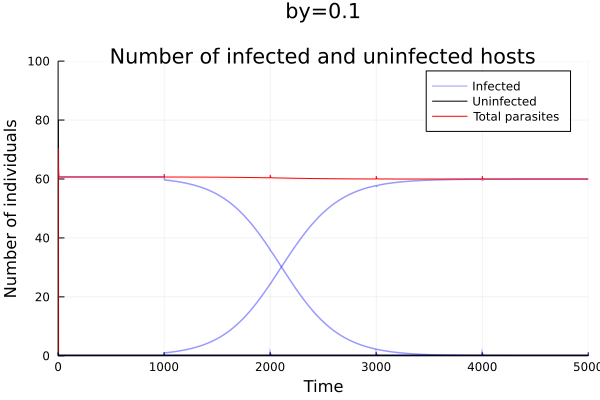
\includegraphics[width=0.4\textwidth]{figures/supp_1a.png}\label{fig:a}}
    \hfil
        \sidesubfloat[]{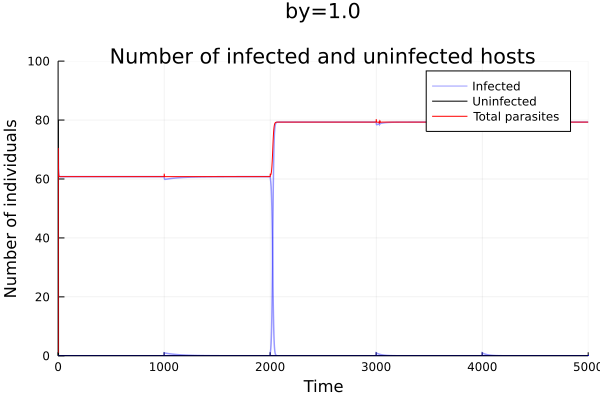
\includegraphics[width=0.4\textwidth]{figures/supp_1b.png}\label{fig:b}}

    \medskip
        \sidesubfloat[]{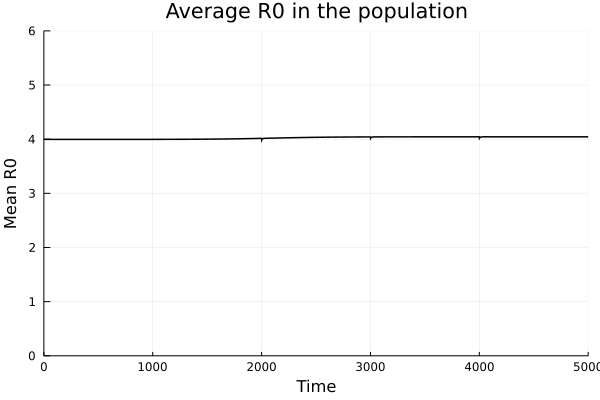
\includegraphics[width=0.4\textwidth]{figures/supp_1c.png}\label{fig:c}}
    \hfil
        \sidesubfloat[]{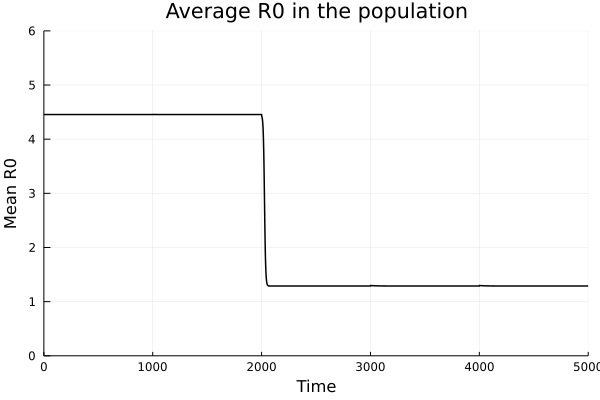
\includegraphics[width=0.4\textwidth]{figures/supp_1d.png}\label{fig:d}}

    \medskip
        \sidesubfloat[]{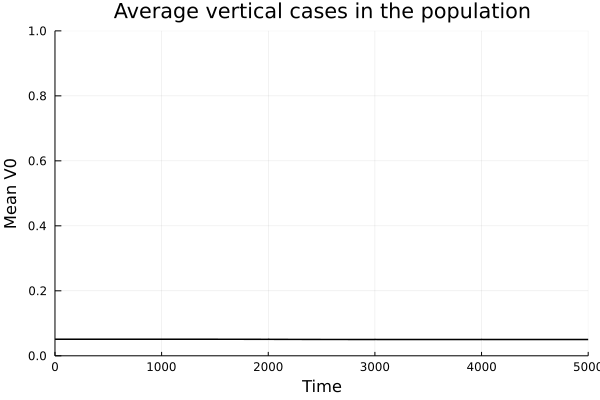
\includegraphics[width=0.4\textwidth]{figures/supp_1e.png}\label{fig:e}}
    \hfil
        \sidesubfloat[]{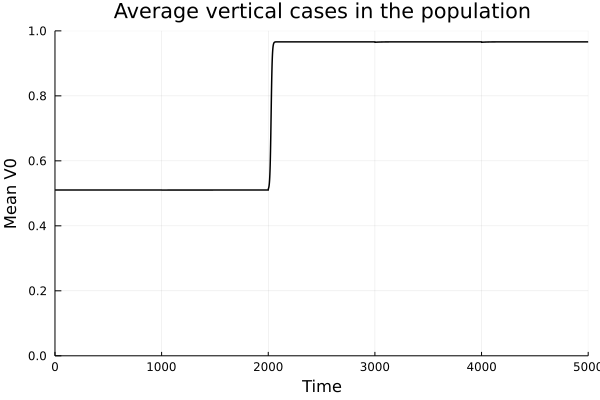
\includegraphics[width=0.4\textwidth]{figures/supp_1f.png}\label{fig:f}}

    \medskip
        \sidesubfloat[]{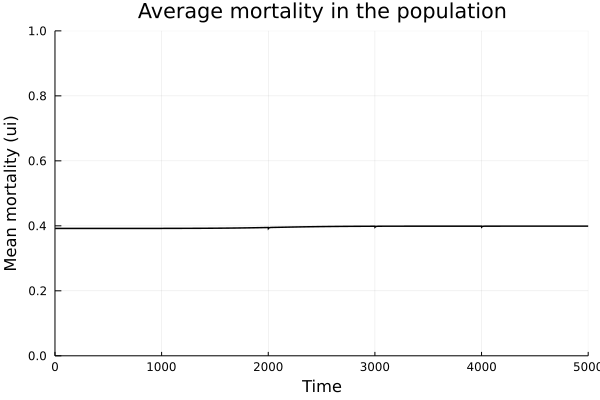
\includegraphics[width=0.4\textwidth]{figures/supp_1g.png}\label{fig:g}}
    \hfil
        \sidesubfloat[]{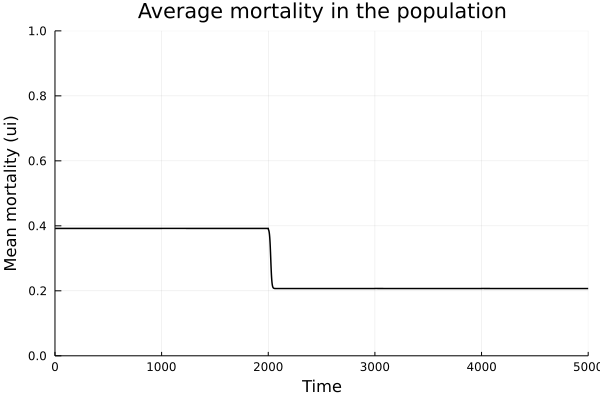
\includegraphics[width=0.4\textwidth]{figures/supp_1h.png}\label{fig:h}}
        
    \medskip
        \sidesubfloat[]{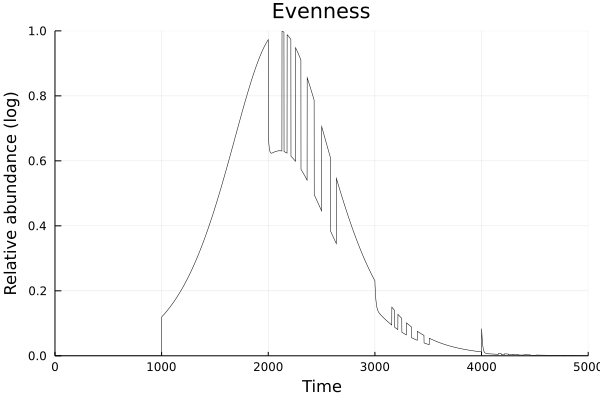
\includegraphics[width=0.4\textwidth]{figures/supp_1i.png}\label{fig:i}}
    \hfil
        \sidesubfloat[]{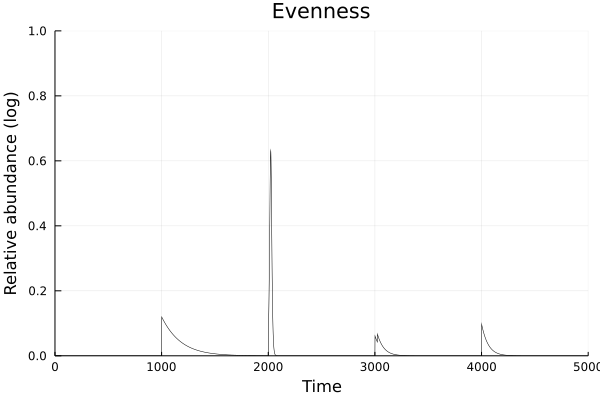
\includegraphics[width=0.4\textwidth]{figures/supp_1j.png}\label{fig:j}}
\caption{Same evolutionary dynamics as seen in Figure \ref{fig:figure1} plotted for 5,000 time-steps only.
}
    \label{fig:SF1}
\end{figure}

\begin{figure}[tbp]
    \centering
        \sidesubfloat[]{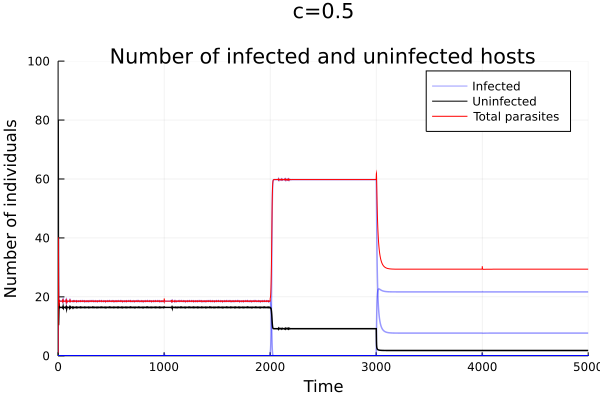
\includegraphics[width=0.4\textwidth]{figures/supp_2a.png}\label{fig:a}}
    \hfil
        \sidesubfloat[]{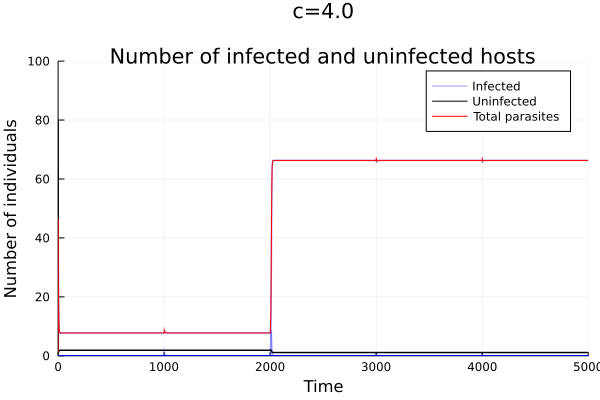
\includegraphics[width=0.4\textwidth]{figures/supp_2b.png}\label{fig:b}}

    \medskip
        \sidesubfloat[]{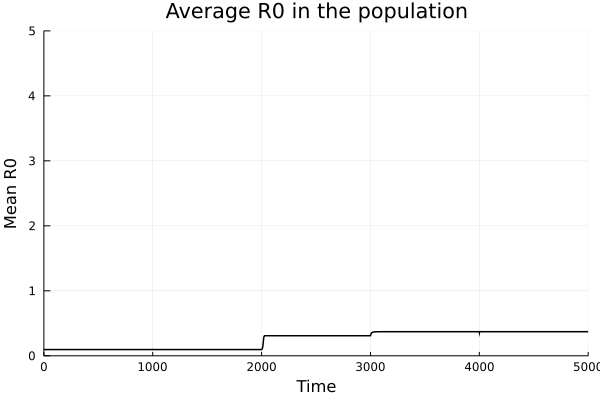
\includegraphics[width=0.4\textwidth]{figures/supp_2c.png}\label{fig:c}}
    \hfil
        \sidesubfloat[]{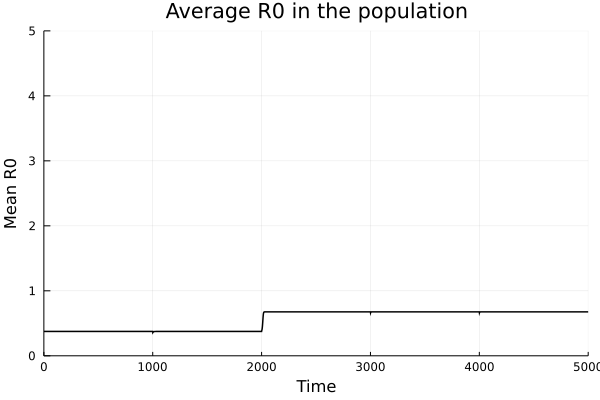
\includegraphics[width=0.4\textwidth]{figures/supp_2d.png}\label{fig:d}}

    \medskip
        \sidesubfloat[]{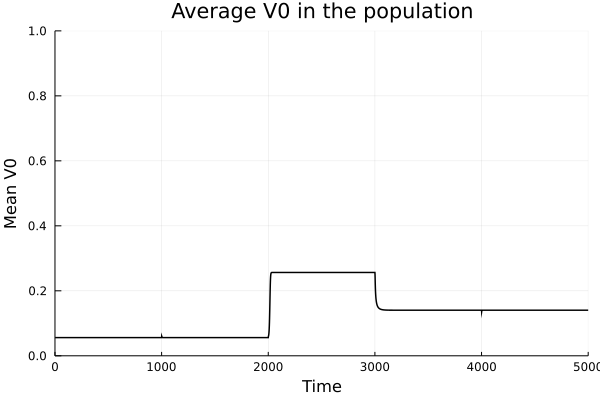
\includegraphics[width=0.4\textwidth]{figures/supp_2e.png}\label{fig:e}}
    \hfil
        \sidesubfloat[]{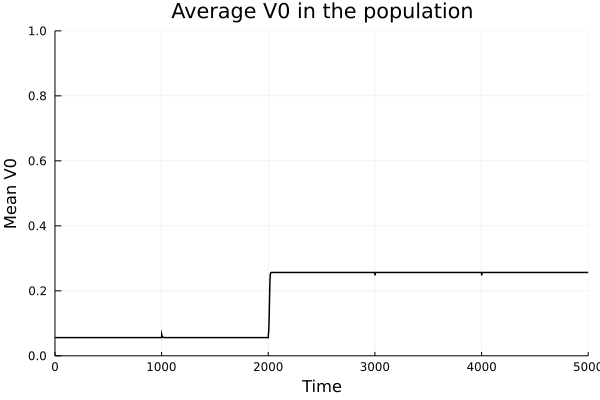
\includegraphics[width=0.4\textwidth]{figures/supp_2f.png}\label{fig:f}}

    \medskip
        \sidesubfloat[]{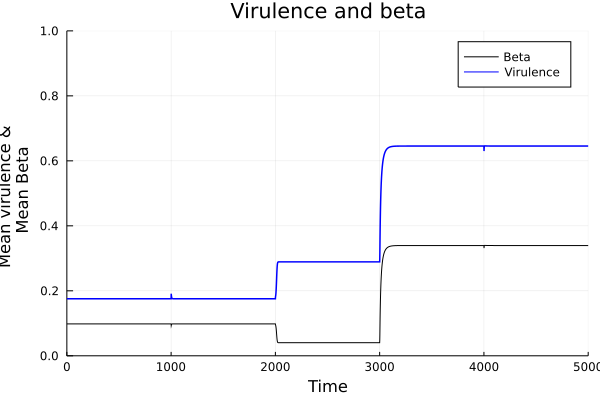
\includegraphics[width=0.4\textwidth]{figures/supp_2g.png}\label{fig:g}}
    \hfil
        \sidesubfloat[]{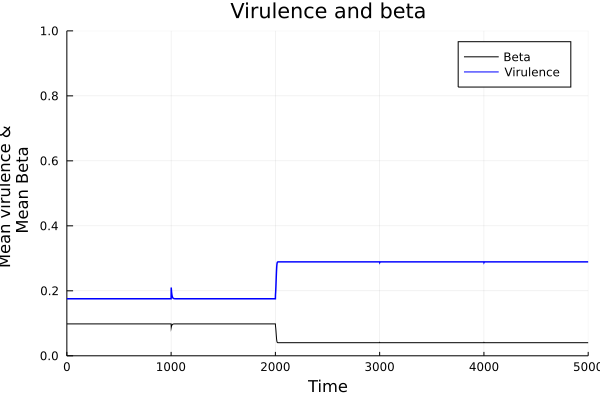
\includegraphics[width=0.4\textwidth]{figures/supp_2h.png}\label{fig:h}}
        
    \medskip
        \sidesubfloat[]{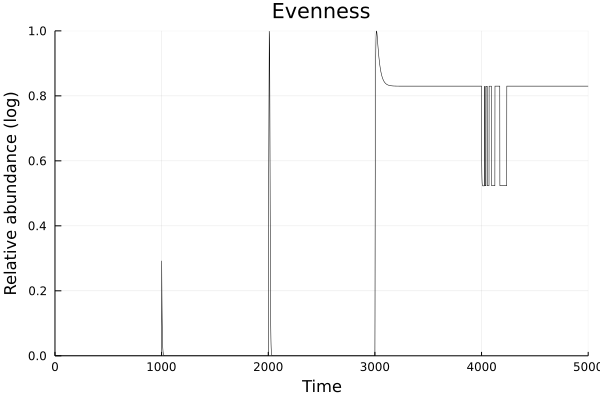
\includegraphics[width=0.4\textwidth]{figures/supp_2i.png}\label{fig:i}}
    \hfil
        \sidesubfloat[]{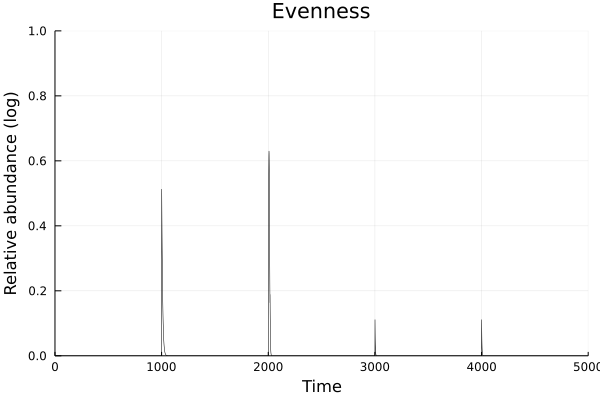
\includegraphics[width=0.4\textwidth]{figures/supp_2j.png}\label{fig:j}}
\caption{Same evolutionary dynamics as seen in Figure \ref{fig:figure2} plotted for 5,000 time-steps only.
}
    \label{fig:SF2}
\end{figure}

\begin{figure}[tbp]
    \centering
        \sidesubfloat[]{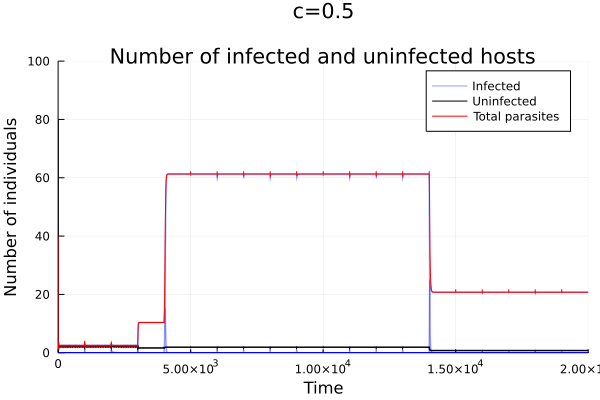
\includegraphics[width=0.4\textwidth]{figures/supp_3a.png}\label{fig:a}}
    \hfil
        \sidesubfloat[]{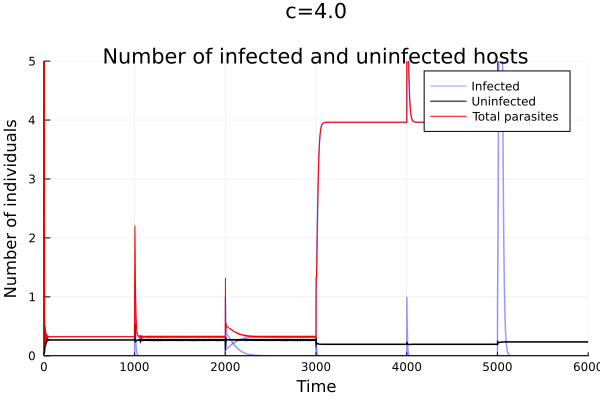
\includegraphics[width=0.4\textwidth]{figures/supp_3b.png}\label{fig:b}}

    \medskip
        \sidesubfloat[]{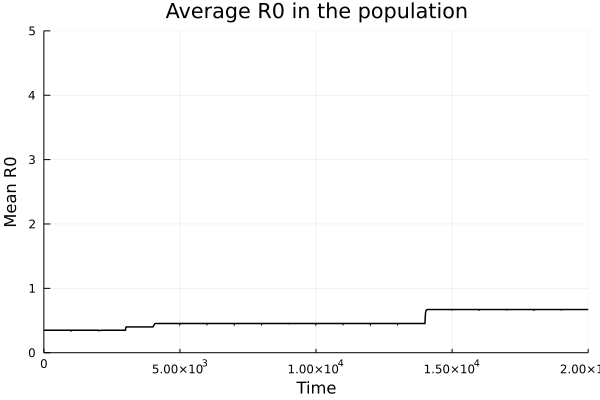
\includegraphics[width=0.4\textwidth]{figures/supp_3c.png}\label{fig:c}}
    \hfil
        \sidesubfloat[]{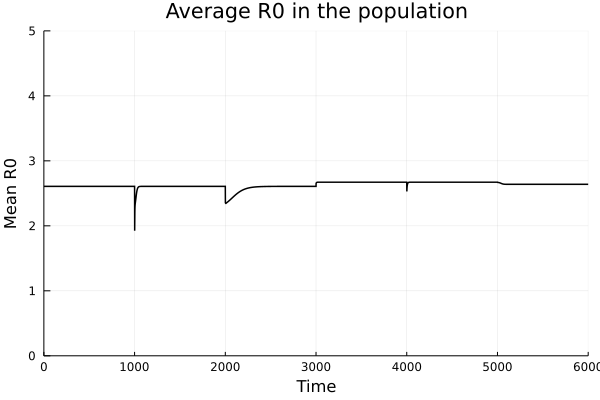
\includegraphics[width=0.4\textwidth]{figures/supp_3d.png}\label{fig:d}}

    \medskip
        \sidesubfloat[]{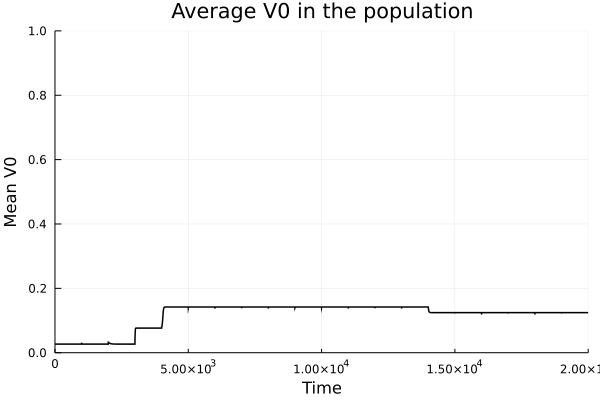
\includegraphics[width=0.4\textwidth]{figures/supp_3e.png}\label{fig:e}}
    \hfil
        \sidesubfloat[]{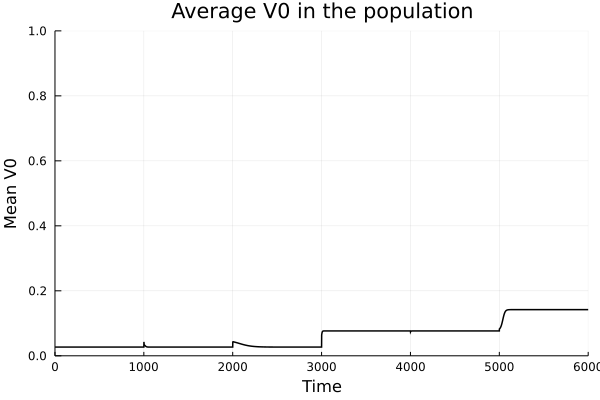
\includegraphics[width=0.4\textwidth]{figures/supp_3f.png}\label{fig:f}}

    \medskip
        \sidesubfloat[]{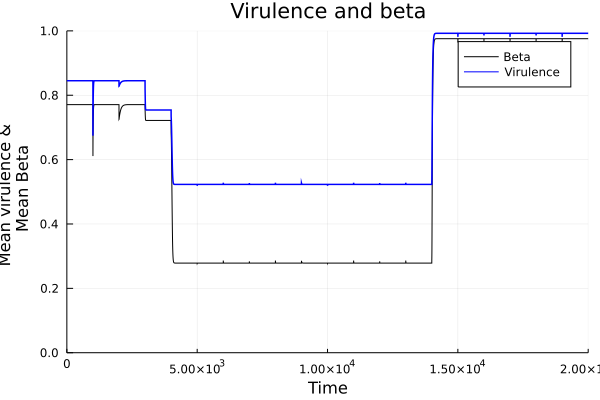
\includegraphics[width=0.4\textwidth]{figures/supp_3g.png}\label{fig:g}}
    \hfil
        \sidesubfloat[]{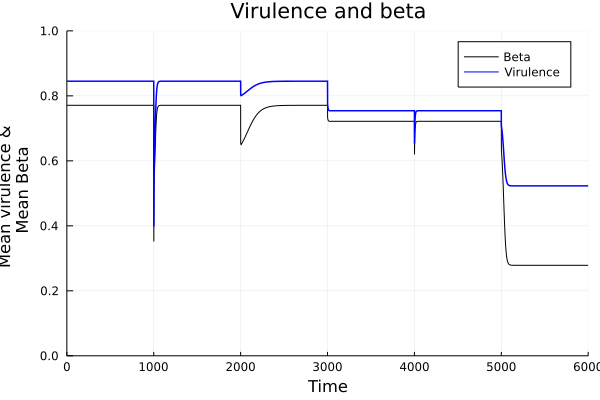
\includegraphics[width=0.4\textwidth]{figures/supp_3h.png}\label{fig:h}}
        
    \medskip
        \sidesubfloat[]{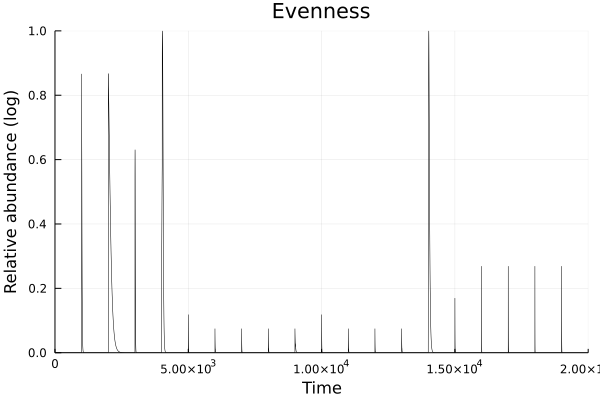
\includegraphics[width=0.4\textwidth]{figures/supp_3i.png}\label{fig:i}}
    \hfil
        \sidesubfloat[]{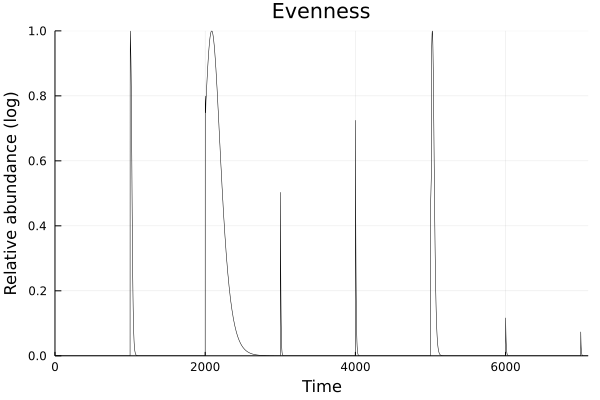
\includegraphics[width=0.4\textwidth]{figures/supp_3j.png}\label{fig:j}}
\caption{Same evolutionary dynamics as seen in Figure \ref{fig:figure3} plotted for only 20,000 and 6,000 time-steps for left and right column, respectively.
}
    \label{fig:SF3}
\end{figure}
